
We classify fragmentation as being either internal or external. Internal fragmentation is considered wasted space due to alignment, which may sometimes be required for an allocator to allocate a slightly larger block of memory than a user has requested. Figure~\ref{fig:internal_fragmentation} shows an example of when a user has requested 100 bytes, where the allocator has instead allocated 128 bytes due to alignment. The last 28 bytes are considered wasted space, or internal fragmentation, as the user will not use them.

\begin{figure}[H]
    \centering
    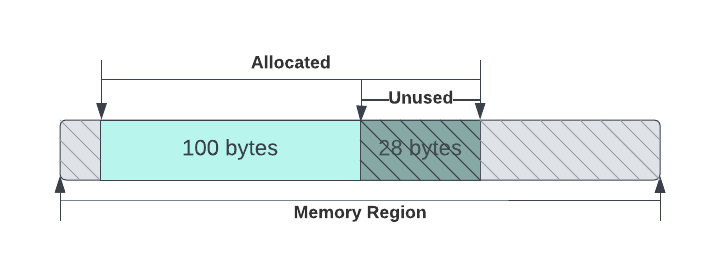
\includegraphics[width=0.75\textwidth]{figures/internal_fragmentation.png}
    \caption{A memory region containing one allocated piece of memory that is 128 bytes large. However, the user only requires 100 bytes of those and thus, 28 bytes is wasted.}
    \label{fig:internal_fragmentation}
\end{figure}

External fragmentation occurs when there is enough memory available in total, but dispersed in smaller, non-contiguous chunks. This is illustrated in Figure~\ref{fig:external_fragmentation}, where a total of 80 bytes is available but distributed across the memory region. Consequently, the user is limited to allocating a maximum of 32 bytes, as the single largest contiguous chunk of memory is of this size.

\begin{figure}[H]
    \centering
    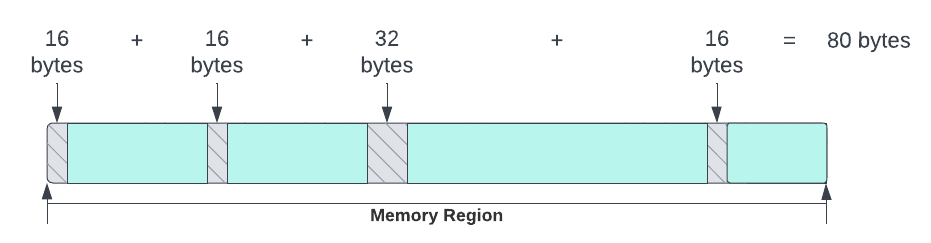
\includegraphics[width=0.8\textwidth]{figures/external_fragmentation.png}
    \caption{A memory region containing several allocated blocks with unused space in between them. Although the total sum of the unused portions is large, a request of more than 32 bytes cannot be fulfilled.}
    \label{fig:external_fragmentation}
\end{figure}

Effectively managing and reducing fragmentation is crucial for optimizing memory usage in long-running programs. Excessive fragmentation can hinder the system's ability to efficiently allocate contiguous blocks of memory for new objects.

%%% Local Variables:
%%% mode: latex
%%% TeX-master: "main"
%%% End:
